
Beim USB-Gadget oder OTG-Betrieb kann die Raspberry Pi Zero direkt �ber den Micro-USB-Anschluss mit einem PC oder Laptop verbunden werden. Er verh�lt sich dann wie ein USB-Ger�t und kann z.~B. ein Massenspeicher-, Serielles-  oder Netzwerkger�t simulieren.\\
Verh�lt er sich als Netzwerkger�t, kann eine Netzwerkverbindung �ber ein virtuelles Netzwerk zum Ger�t hergestellt werden. 
Weitere Informationen �ber den OTG-Betrieb kann der Git-Hub Seite  \url{https://gist.github.com/gbaman/50b6cca61dd1c3f88f41} entnommen werden.

\subsection{Client - Raspberry Pi Zero}

Nach der Einrichtung des Betriebssystems auf der MicroSD-Karte m�ssen noch ein paar Modifikationen an den Dateien der Boot-Partition durchgef�hrt werden. 

Folgender Text muss nach der Anweisung "`rootwait"' in die Datei "`cmdline.txt"' eingef�gt werden:
\begin{screensmall}
modules-load=dwc2,g_ether g_ether.host_addr=00:01:02:03:04:05 g_ether.dev_addr=00:01:02:03:04:06
\end{screensmall}

Die Angabe der MAC-Adresse f�r Host und Ger�t ist optional, es wird aber empfohlen, da sonst diese Adressen zuf�llig vergeben werden. Die Werte k�nnen frei gew�hlt werden, sollten sich aber nicht mit den Adressen im Netz bzw. Host �berschneiden.\\

Folgende Zeile muss am Ende in die Datei "`config.txt"' hinzugef�gt werden:
\begin{screensmall} 
dtoverlay=dwc2
\end{screensmall}

Weiters muss eine leere Datei mit dem Namen "`ssh"' erzeugt werden, damit der SSH-Dienst automatisch nach dem Start ausgef�hrt wird. Danach kann die MicroSD-Karte in den Raspberry Pi Zero gesteckt und �ber ein MicroUSB-Kabel an einen Computer angeschlossen werden. 
Es ist zu beachten, dass das MicroUSB-Kabel am mittleren MicroUSB-Anschluss angeschlossen werden muss!\\

%\begin{console} 
%	touch /mnt/ssh
%\end{console} 

%Wird Microsoft Windows verwendet so muss das Programm Bonjour von Apple installiert werden. 
%Falls der Dienst noch nicht von einem Apple Programm (iTunes oder Quicktime) installiert wurde, kann von der Seite \url{https://support.apple.com/kb/DL999?locale=de_AT} ein Setup heruntergeladen werden.\\

\subsection{Host - Kubuntu 16.04 (Zeroconf)}

Die Konfiguration der IP-Adressen erfolgt �ber das Zero Configuration Networking System (Zeroconf). Dazu muss am Host-PC der Dienst Avahi (avahi-daemon) installiert sein. Dieser ist auf den meisten Linux Systemen bereits vorinstalliert.\\ 
  
Zur Konfiguration unter Linux Kubuntu 16.04 muss zuerst "`Netzwerkverbindungen"' ge�ffnet werden. 
Dazu klickt man mit der rechten Maustaste auf das Netzwerksymbol in Infobereich rechts unten. Nun kann die Option "`Netzwerkverbindungen einrichten..."' ausgew�hlt werden.

\begin{figure}[ht]
  \centering
  
\includegraphics[scale=1.0]{images/OTG_NetzwerkverbindungenIcon.png}	
  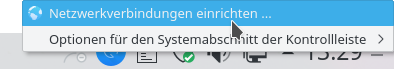
\includegraphics[scale=0.42]{images/OTG_NetzwerkverbindungenOpen.png}	
  %	\caption{}
  \label{OTG_LINUX_NetzwerkverbindungenApp}
\end{figure}


Danach kann die neue "`Kabelnetzwerkverbindung"' umbenannt werden, z.~B. in Raspberry Pi Zero. Erkennen kann man das Netzwerk an der Mac-Adresse die man bei "`g\_ether.host\_addr"' angegeben hat (z.~B. 00:01:02:03:04:05).  


\begin{figure}[ht]
  \centering
  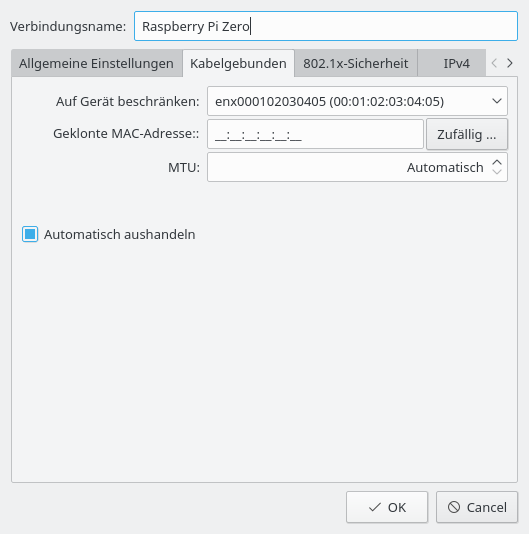
\includegraphics[scale=0.45]{images/OTG_Pi_Verbindungsname.png}
	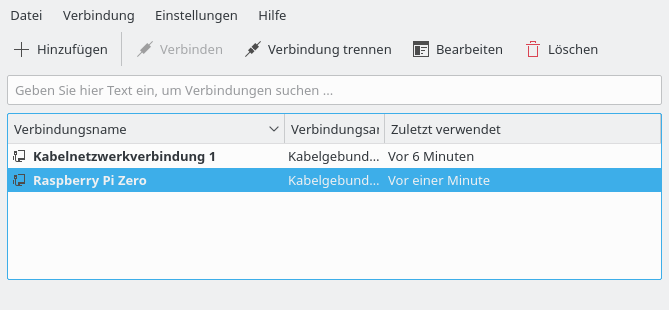
\includegraphics[scale=0.45]{images/OTG_Netzwerkverbindungen.png}
%	\caption{}
  \label{OTG_LINUX_Netzwerkverbindungen}
\end{figure}


Am Host-PC muss bei den IPv4-Einstellungen Methode "`Link-Local"' eingestellt sein.  


\begin{figure}[ht]
  \centering
  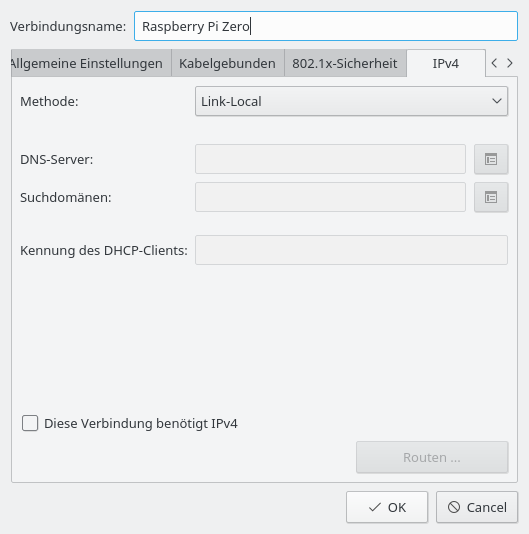
\includegraphics[scale=0.45]{images/OTG_IPv4.png}
%	\caption{}
  \label{OTG_LINUX_IPV4}
\end{figure}


%\subsection{Internet Zugriff} 
~\\
Nach der Einrichtung des Netzwerk kann der Raspberry Pi Zero mit dem Namen "`raspberrypi.local"' erreicht werden. Um den Raspbery Pi Zero mit dem Internet verbinden zu k�nnen m�ssen einige Einstellungen am Host %und Client
 gemacht werden. Man muss den Name des Netzwerkger�ts am Host-PC kennen, das mit dem Internet verbunden ist. Dies ermittelt man �ber die Netzwerkeinstellungen oder �ber die Konsole mit nmcli. Im Beispielfall ist der Name "`enp0s25"' das richtige Ger�t.

\begin{console} 
	nmcli d
\end{console} 

\begin{screensmall} 
	GER�T            TYP       STATUS           VERBINDUNG        
	enx000102030405  ethernet  verbunden        Raspberry Pi Zero 
	enp0s25          ethernet  verbunden        Netzwerkverbindung 1                
	lo               loopback  nicht verwaltet  --  
\end{screensmall}

Damit der Internetzugang f�r den Raspberry Pi Zero freigegeben wird, m�ssen am Host-PC folgende Befehle in einem Terminal eingeben werden. "`enp0s25"' muss durch den Namen des Netzwerkger�ts ersetzt werden, das mit dem Internet verbunden ist.

\begin{console} 
	sudo sysctl -w net.ipv4.ip_forward=1
	sudo iptables -t nat -A POSTROUTING -o enp0s25 -j MASQUERADE
\end{console}



Sp�ter wird noch die IP-Adresse der lokalen Raspberry Pi Verbindung ben�tigt. Dies ermittelt man in der Konsole mit dem Befehl \texttt{ifconfig}.  

\begin{console} 
	ifconfig enx000102030405 | head -n 2
\end{console}

\begin{screensmall} 
	enx000102030405 Link encap:Ethernet  Hardware Adresse 00:01:02:03:04:05  
	inet Adresse:169.254.144.15  Bcast:169.254.255.255  Maske:255.255.0.0
\end{screensmall}


